\documentclass[conference]{IEEEtran}
\IEEEoverridecommandlockouts
% The preceding line is only needed to identify funding in the first footnote. If that is unneeded, please comment it out.
\usepackage[style=ieee, backend=biber]{biblatex}
\addbibresource{references.bib}
\addbibresource{ai_citations.bib}
\usepackage{amsmath,amssymb,amsfonts}
\usepackage{algorithmic}
\usepackage{graphicx}
\usepackage{textcomp}
\usepackage{xcolor}
\def\BibTeX{{\rm B\kern-.05em{\sc i\kern-.025em b}\kern-.08em
    T\kern-.1667em\lower.7ex\hbox{E}\kern-.125emX}}
\begin{document}

\title{Human-Centered Intelligent Robots: A Literature Review\\
% \thanks{Identify applicable funding agency here. If none, delete this.}
}

\author{\IEEEauthorblockN{1\textsuperscript{st} Srijan Prasad Joshi}
\IEEEauthorblockA{\textit{Dept.\ of Computer Science} \\
\textit{Ramapo College of New Jersey}\\
Mahwah, United States of America \\
sjoshi3@ramapo.edu}
\and
\IEEEauthorblockN{2\textsuperscript{nd} Prerak Pandey}
\IEEEauthorblockA{\textit{Dept.\ of Computer Science} \\
\textit{Ramapo College of New Jersey}\\
Mahwah, United States of America \\
ppandey@ramapo.edu}
}

\maketitle

\begin{abstract}
Intelligent robots are becoming more and more mainstream. Tools such as Google voice assistant, becoming an integral part of many people's lives. As such, human-centered intelligent robot has become an important research field that spans across all fields in robotics such as intelligent control and path navigation. In this paper, we present the recent achievements of human-centered robotics and analyze the contemporary academic literature of this field. Furthermore, we look at the issues we had in the past, demonstrate why the recent approaches solved them, and discuss what the challenges that contemporary research are tying to solve in this field.
\end{abstract}

\begin{IEEEkeywords}
Human-centered robots, anthropomorphism, pattern recognition, computer vision, natural language processing, path planning, past issues, cloud based computing, computer hardware, intelligent control, navigation
\end{IEEEkeywords}

\section{Introduction}
Humanoid robots are very popular in science fiction. There are many movies such as the terminator where the robots are almost identical to humans. In the past two decade big progress has been made to make robots increasingly human. Compared to traditional robots such as industrial robots, human-centered robots require completely different performance measurement requirements\autocite{zinn2004new}. In this paper, we will present the various driver of this anthropomorphic development in robotics and delve into the literature that analyzes the contemporary research in them.

\section{Pattern Recognition}
The human brain has the capability to recognize various patterns to function. As such, we would want an anthropomorphic robot to use mimic this useful ability. In the past decade much progress has been made in this area of robotics given the rapid expanse of artificial intelligence. One main impetus for progress in pattern recognition is the rise of GPU accelerated machine learning techniques. One popular technique on the rise for pattern recognition is reinforcement learning where an agent uses many types of reinforcement learning which tries to maximize some sort of reward function for the agent. This sort of approach utilities mathematical models that uses. One common type of machine learning model used in robotics is the artificial neural network. However, though these have been proved to be very useful and though their distributed nature is similar to natural neural networks, their name itself is misleading because they have flaws like being brittle, inefficient, and myopic\autocite{Watson2019}. Though there are many projects that have used artificial neural networks to achieve very anthropomorphic results. One such project is famous alpha go project that used artificial neural networks to create an AI that beat Lee Sedol in a 6 game match against alpha go\autocite{silver2017mastering}. In that project, the neural network was initially trained using human game datasets and was then later trained using dataset of its own games\autocite{silver2017mastering}. Another project that was inspired from this project was a table tennis playing robot by \textcite{lin2020}. In that project, \textcite{lin2020} used Deep Neural Networks to handle parameters such as air resistance, the magnus effect, etc., and trained the said network using real life game simulations.

\subsection{Computer Vision}
wiley2018computer
One of the key driving factors of intelligent robots is the progress that we have made in computer vision in the past decade. Computer vision has been expanded into the vast area of field ranging from recording raw data into the extraction of image pattern and information interpretation\autocite{patel2012machine}. Most of the tasks in computer vision are related to observing input scenes and getting the necessary information from them. ``Computer vision works by using an algorithm and optical sensors to stimulate human visualization to automatically extract valuable information from an object''\autocite{wiley2018computer}. This field has been studied from many different perspectives and combines ideas from digital image processing, pattern recognition, machine learning, computer graphics, and human neurology. 

During the 1990s, there was not much progress made in this field. However, ever since \textcite{krizhevsky2012imagenet} published their paper on Alexnet and demonstrated their groundbreaking result on image classification using CNNs and GPU accelerated deep learning, there has been a boom in the future papers utilizing such tools. Robots now are capable of performing various forms of vision tasks that they were previously unable to perform. One famous modern application is in unmanned vehicles where the vehicle is able to navigate around its environments simply with the usage of visual data. Another is medical image processing where machine help medical professionals get information about patients from visual data. This boom in computer vision is so significant it even leads \textcite{pratt2015cambrian} to call it the possible ``robotics Cambrian explosion'' because this phenomenon of robotic achieving vision is just like the era when there was an exponential increase in evolutionary diversity largely caused by the natural creatures gaining vision. 


\subsection{Natural Language Processing}
Another area of artificial intelligence that is engendering anthropomorphic robots is the area of natural language processing. We as human beings have the most complex systems of utilizing natural sounds among any living creatures. We can form several different patterns and use sounds in complex ways to convey and understand information. As such, we would expect humanoid robots to be capable of handling such languages. The area of natural language processing is a branch of artificial intelligence that deals with the interaction between machines and humans using the natural language. This field just like computer vision has grown very big. In recent years we see exemplary tools such as Google translate and home assistant that have been made possible thorough natural language processing. According to \textcite{hirschberg2015advances} the main reasons for this are (i) increase in computing power (ii) availability of large amounts of linguistic data (iii) success of machine learning (iv) richer understanding of the structure of human language and its deployments in social contexts. The big progress done in this subfield are in machine translation (translating one language to another), spoken dialog systems and conversational agents (agents generating and interpreting human voice; e.g. Google assistant, Apple's Siri) and machine reading (the ability to interpret human written texts)\autocite{hirschberg2015advances}.

\section{Computer Hardware}
Moore’s law states that the number of transistors on a microprocessor chip will double every two years or so -- which has generally meant that the chip's performance will too\autocite{waldrop2016chips}. This has generally been true for the past several decades although  it is now encountering some fundamental physical limits. Semiconductor comanies are now manufacturing transistors on chips that are on a scale of 14 nanometers\autocite{pratt2015cambrian}. This small scale approach is reaching physical limit because of how close these transistor sizes are getting to the atomic level\autocite{waldrop2016chips}.

Furthermore, the usage of GPU accelerated has greatly expedited the speed that algorithms can run on. GPU or Graphics Processing Units made by NVIDIA or AMD were originally designed to be components in graphics subsystems. However, in the two few decades machine learning algorithms have greatly benefited from this hardware. Given the multi-threaded nature of GPUs, they act as the optimal option to perform matrix operations on\autocite{steinkraus2005using}. These matrix operations are at the heart of many machine learning algorithms. Fox example, the gradient descent algorithm in an artificial neural network could be thought of as a collection of matrix multiplications\autocite{krizhevsky2012imagenet}. The results that we are seeing from these new machine learning algorithms would have not been possible with the traditional single threaded CPU because executing single sequential instructions instead of multiple parallel instruction is much slower. 

Also, not just the improvement in computational speed, but even the readily available semiconductors are a large cause for the development of modern robotics. It is much cheaper to get the necessary tools required to build a robot in 2021 than it was ten or twenty years ago. This has significantly contributed to the increase research works in intelligent robots.

\section{Human-Robot Interactions}
\begin{figure}[h]
    \centerline{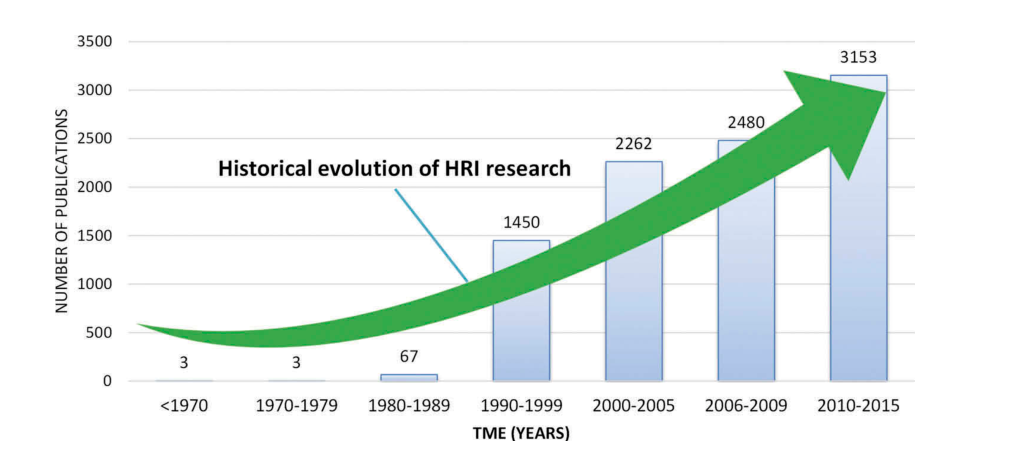
\includegraphics[width=0.5\textwidth]{images/evolution_of_hri.png}}
    \caption{Figure showing the increase in the publications related to HRI from 1960 - 2015. Figure gotten from\autocite{tsarouchi2016human}}
\label{fig1}
\end{figure}

\begin{figure}[h]
    \centerline{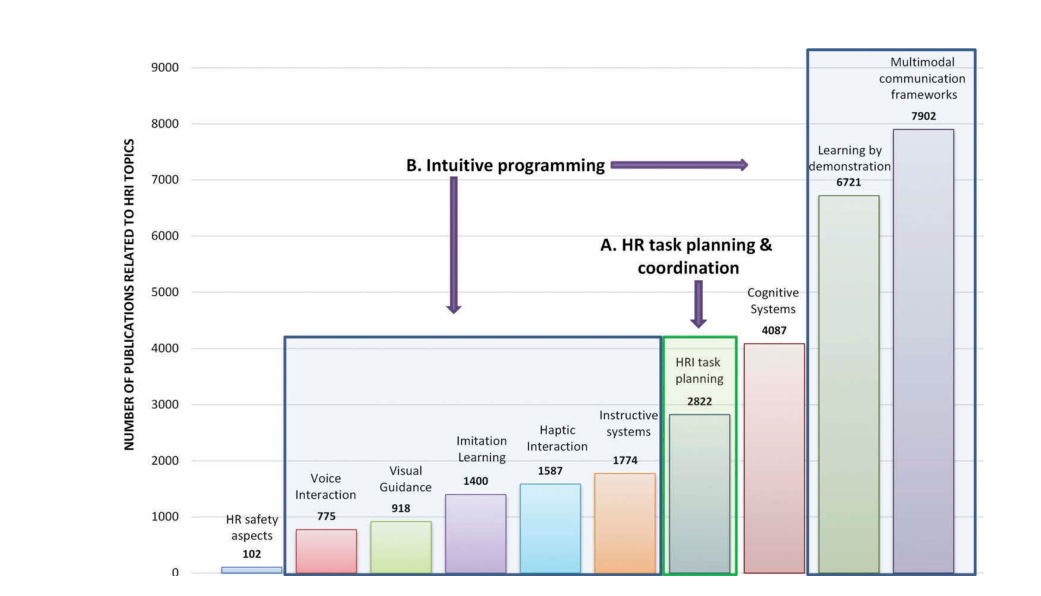
\includegraphics[width=0.5\textwidth]{images/hri_total_number_of_publication.png}}
    \caption{Figure showing the total number of publications from 1970-2015 within per aspect of HRI. The two most dominating subfields are ``Learning by demonstration'' and ``Multimodal communication frameworks''. Figure gotten from \autocite{tsarouchi2016human}}
\label{fig2}
\end{figure}

Human-robot interaction is an expanding field with hundreds of publications being published each year by many different professional societies (as shown in figure \ref{fig1}). \textcite{sheridan2016human} states that HRI can be roughly divided into four areas of application: Human supervisory control of robots in performance of routine tasks; Remote control of space, airborne, terrestrial, and undersea vehicles for non-routine tasks in hazardous or inaccessible environments, automated vehicles in which a human is a passenger, and Human–robot social interaction. 
\begin{itemize}
\item \textbf{Human supervisory control of robots in performance of routine tasks:} This area deals with handling parts on manufacturing assembly lines and the delivery of packages, components, mail, and medicines in warehouses, offices and hospitals\autocite{sheridan2016human}. Human operators are required to supervise the use of such machines and it is an important area in intelligent robotics. There are still much research being Safety is a big concern in this subfield.
\item \textbf{Remove control of Vehicles:} Robots being needed to operate in hazardous areas and not endanger humans to such places were one of the primary motivators of early robotics development.Much progress has been made in remote control of unmanned spacecraft, undersea robotic vehicles, and unmanned aerial vehicles. Human factors research continues to be needed for improving and simplifying display and control interfaces\autocite{sheridan2016human}. There are promising developments in using robotic avatars for surveillance, search and rescue for police work, border patrol, firefighting and rescue, and military operations, with many human factor issues for display and control and mental workload\autocite{sheridan2016human}.
\item \textbf{Automated Vehicles With Human Passenger:} One famous new technology that arouses much excitement is the new driverless vehicles. ``As is well known, recently Google has produced a self-driven car, demonstrated successfully on California freeway''\autocite{sheridan2016human}. This area has certainly gotten more and more successful these past ten years. However, one large safety issue in this field is the human driver not staying alert and take over should the automation fail. We already have minimized the error rate to to less that 0.1 percent. However, this is still considered too large for this technology to be utilized in the mainstream.
\item \textbf{Human-Robot Social Interactions:} Robots functioning in social situations and becoming more anthropomorphic is a big part of human-robot interactions. We want humanoid robots to be able to demonstrate the same social abilities as humans and participate in social situations competently. The Sophia bot developed by Hanson AI is a famous example that is capable of mimicking human facial expressions and speech patterns.
\end{itemize}


\section{Major Contemporary Challenges}
\begin{figure}[h]
    \centerline{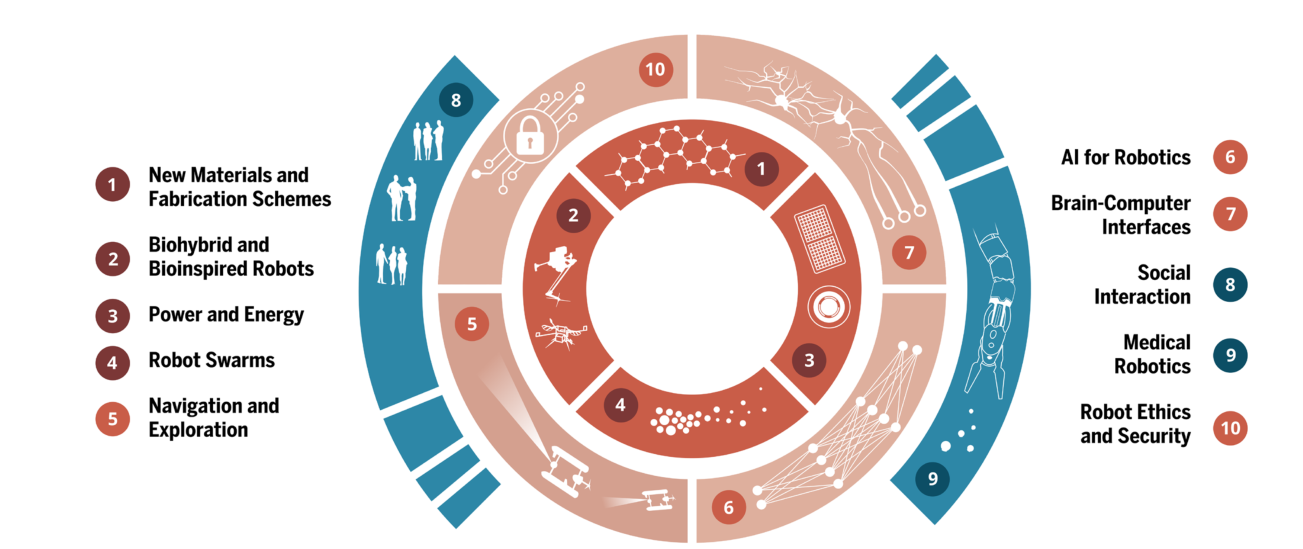
\includegraphics[width=0.5\textwidth]{images/grand_challenges.png}}
    \caption{Figure showcasing the challenges big challenges to modern robotics. Figure gotten from\autocite{yang2018grand}}
\label{fig3}
\end{figure}
In the paper "The grand challenges of Science Robotics", the authors \textcite{yang2018grand} mention the following as the biggest challenges to future robotics for the next 5 - 10 years. They can easily be interpolated to human-centered robots as well.
\begin{itemize}
\item \textbf{Robot swarms:} Emergence is one of the most interesting observations we see in our natural environment. Robots swarms replicate natural emergence and allow simpler, less expensive, modular robotic units to be reconfigured into a team. Robot networks integrated with our infrastructure have tremendous potential for solving the most pressing problems facing human civilization. 
\item \textbf{Brain-computer interfaces:} A brain-computer interface forms a direct connection between the human brain and machine. ``Direct use of brain activity to control a computer or external device without the mediation of the peripheral, somatomotor nervous system has major applications in enabling paralyzed patients to communicate and control robotic prosthetics and in rehabilitation for restoring neural function''\autocite{yang2018grand}. However, in this field there are challenges like sensing and acquiring acquisition being cumbersome, data processing and dealing with artifacts of non cerebral origin, particularly for wearable approaches, and finding out if BCI will ever outperform simpler techniques like eye tracking or muscle based devices.
\item \textbf{Social interaction:}Because humans are so adept at recognizing and interpreting social behavior, we often underestimate the complexity of the challenge that this represents for a robot. Social interaction is a major challenge for robotics in part because the perceptual demands are so significant. Social cues—such as gaze direction, facial expressions, or vocal intonation—are often extremely detailed. There are many details to consider for robot can appropriately evaluate social these cues and act accordingly. This is certainly a big challenge in this field.
\item \textbf{New Materials and their fabrication schemes:} Gears, motors, and mechanical actuators have always been the use in many robotic projects. However, newer generation of robots are exploring ``new materials including artificial muscles, compliant materials for soft robots, and emerging advanced manufacturing and assembly strategies''\autocite{yang2018grand} These new genre of materials are power efficient, multi functional, compliant, and autonomous in ways that are similar to biological organisms. ``However, most demonstrations using new materials and fabrication strategies have been “one-offs” and must still overcome basic hurdles to achieve wide-scale adoption''\autocite{yang2018grand}. 
\item \textbf{Bioinspired and biohybrid robots:} Bioinspired robotics in our context means the  use of fundamental biological principles that are translated into engineering design rules for creating robots. If the biological understanding results in the direct use of biological material to design synthetic machines, then our context refers to this as a biohybrid robot. For biohybrid and bioinspired robots, actuation and energy remain major bottlenecks compared with performance seen in animals. As bioinspired robots venture beyond the laboratory, models of real-world, unstructured environments will be required, but none can yet adequately represent our complex, dynamic world
\item \textbf{Navigation and exploration:} Though we have achieve a lot in term of navigation, there are still challenges in this area. One is that robots struggle to operate in environments that are unmapped and when the environment's nature is not understood\autocite{yang2018grand}. For navigation, the grand challenge is to handle failures and being able to adapt, learn, and recover. For exploration, it is developing the innate abilities to make and recognize new discoveries.
\item \textbf{Fundamental aspects of artificial intelligence for robotics:} The advent of deep learning methods resulted in remarkable levels of object recognition accuracy (61) using hierarchical pattern recognition that retained information coherence at each level of the hierarchy. However, we still are not anywhere near reaching the intelligence that we see in humans.
\item \textbf{Ethics and security:} With increasing levels of autonomy and humanrobot interaction, there needs to be careful consideration of potential regulatory, ethical, and legal barriers and the context of how robots are deployed. Technologies like STARRA are projected become more and more commonplace in the workforce. As such, there are many ethical question that comes up in regards to utilizing these machines as we progress to the future. The field of ethics and security is an important field for robotics and AI.
\end{itemize}

\newpage{}
\printbibliography{}
\end{document}
